\section{The Effects of Ties}

\paragraph{Problem} 
Repeated forward a* needs to break ties to decide which cell to expand next if
several cells have the same smallest f-value. It can either break ties in favor
of cells with smaller g-values or in favor of cells with larger g-values.
implement and compare both versions of repeated forward a* with respect to
their runtime or, equivalently, number of expanded cells. Explain your
observations in detail, that is, explain what you observed and give a reason
for the observation.

\paragraph{Solution} 
After running two algorithms respectively for 50 random maps of size $101\times
101$ (with discrete obstacles), the result is shown in table \ref{tbl:two-rpa}.
(Please refer to appendix a for full list of results.)

\begin{table}[h!]
\centering
\caption{Result of two Repeated Forward A* algorithms}
\begin{tabular}{|l|l|l|l|l|}
\hline
Algorithm & Aver. Expa/M & aver. Expa/P & Aver. Expl/M & Aver. Expl/P \\
\hline
Raw RFA* & 264141.78 & 3058.58 & 285757.42 & 3308.32 \\
\hline
Modified RFA* & 8847.88 & 92.44 & 25461.42 & 267.68 \\
\hhline{|=|=|=|=|=|}
Algorithm & Aver. Moves & Aver. Count & Aver. Optimal & Aver. Ratio \\
\hline
Raw RFA* & 335.72 & 88.2 & 198.6 & 1.6852 \\
\hline
Modified RFA* & 367.56 & 96.04 & 198.6 & 1.8458 \\
\hline
\end{tabular}
\label{tbl:two-rpa}
\end{table}

In the table, raw RFA* is the RFA* algorithm that breaks ties by $f$ value and
the modified RFA* is the one that breaks ties by $c\times f-g$. the meaning of
each column is listed as below:

\begin{itemize}
\item Expa/M: total number of cells expanded in each map;
\item Expa/P: average number of cells expanded in each plan;
\item Expl/M: total number of cells explored in each map;
\item Expl/P: average number of cells explored in each plan;
\item Moves: total number of actual moves in each map;
\item Count: total number of planning in each map;
\item Optimal: number of optimal (minimum) moves in each map;
\item Ratio: ratio of moves/optimal;
\end{itemize}

As we can see, the average number of cells expanded in each map by raw RFA* is
almost 30 times as that by modified RFA*. Similarly, the average number of
cells expanded at each planning (call computepath) by raw RFA* is also 33 times
as that by modified RFA*. This indicates that modified RFA* expands much less
cells than that by modified RFA*. This is similar to the number of explored
cells, which represents all the cells that are added to $open$ list and some of
them may not be extracted to expand. We can see that the average number of
explored in each map by raw RFA* is more than 10 times as that by modified
RFA*, and ratio of the number for each planning reaches over 12 times. However,
when we inspect the average number of moves, the situation is quite different.
Thanks to the large-scale nodes expanded, raw RFA* enable agent to move nearly
9\% less steps than modified RFA* either in each map or for each planning. This
indiates that the move part of raw RFA* is more likely to approach optimal.

To explain in detail, let's introduce a simple example as shown in figure
\ref{fig:p2-example}. It is a $5\times 5$ grid map where the start cell is at
$(A,1)$ and the goal cell is at $(E,5)$.  We can see that raw RFA* in Figure
\ref{fig:rawforward} almost expands all cells on the map while modified RFA* in
Figure \ref{fig:newforward} only expands some useful cells. The reason for this
difference depends on the way they break ties. In Figure \ref{fig:rawforward},
the algorithm only use $f$-value to determine the order of expansion which
causes a lot of tie cases. For example, at first, the agent will explore its
neighbors $(A,2)$ and $(B,1)$, whose $g$-values are both set as 1, $h$-values
are 7 and $f$-values are 8. The next node to expand is either $(A,2)$ or
$(B,1)$, so without loss of generality, let's pick $(B,1)$. After that, cell
$(C,1)$ is explored whose $g=2$, $h=6$ and $f=8$. (Just forget $(B,2)$
temporarily.) It has the same $f$-value as $(A,2)$.  In this case, raw RFA*
will pick one arbitrarily, and if it picks $(A,2)$, $(A,3)$ will be explored.
But for modified RFA*, it will inspect $g$ value to break ties between $(A,2)$
and $(C,1)$ and pick the cell with smaller $g$, that is $(C,1)$. Repeatedly,
modified RFA* will expand much less cells than raw RFA*. Therefore, this is the
effect of breaking ties by using $c\times f-g$ value.

\begin{figure}[t]
  \centering
  \begin{subfigure}[b]{0.35\textwidth}
    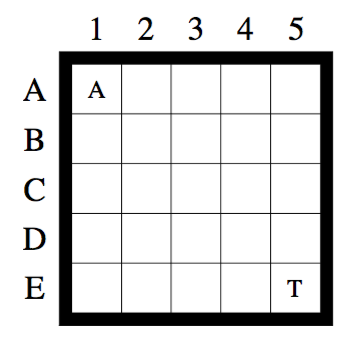
\includegraphics[width=\textwidth]{p2-example}
    \caption{Third Example of Search Problem}
    \label{fig:p2-example}
  \end{subfigure}
  ~
  \begin{subfigure}[b]{0.30\textwidth}
    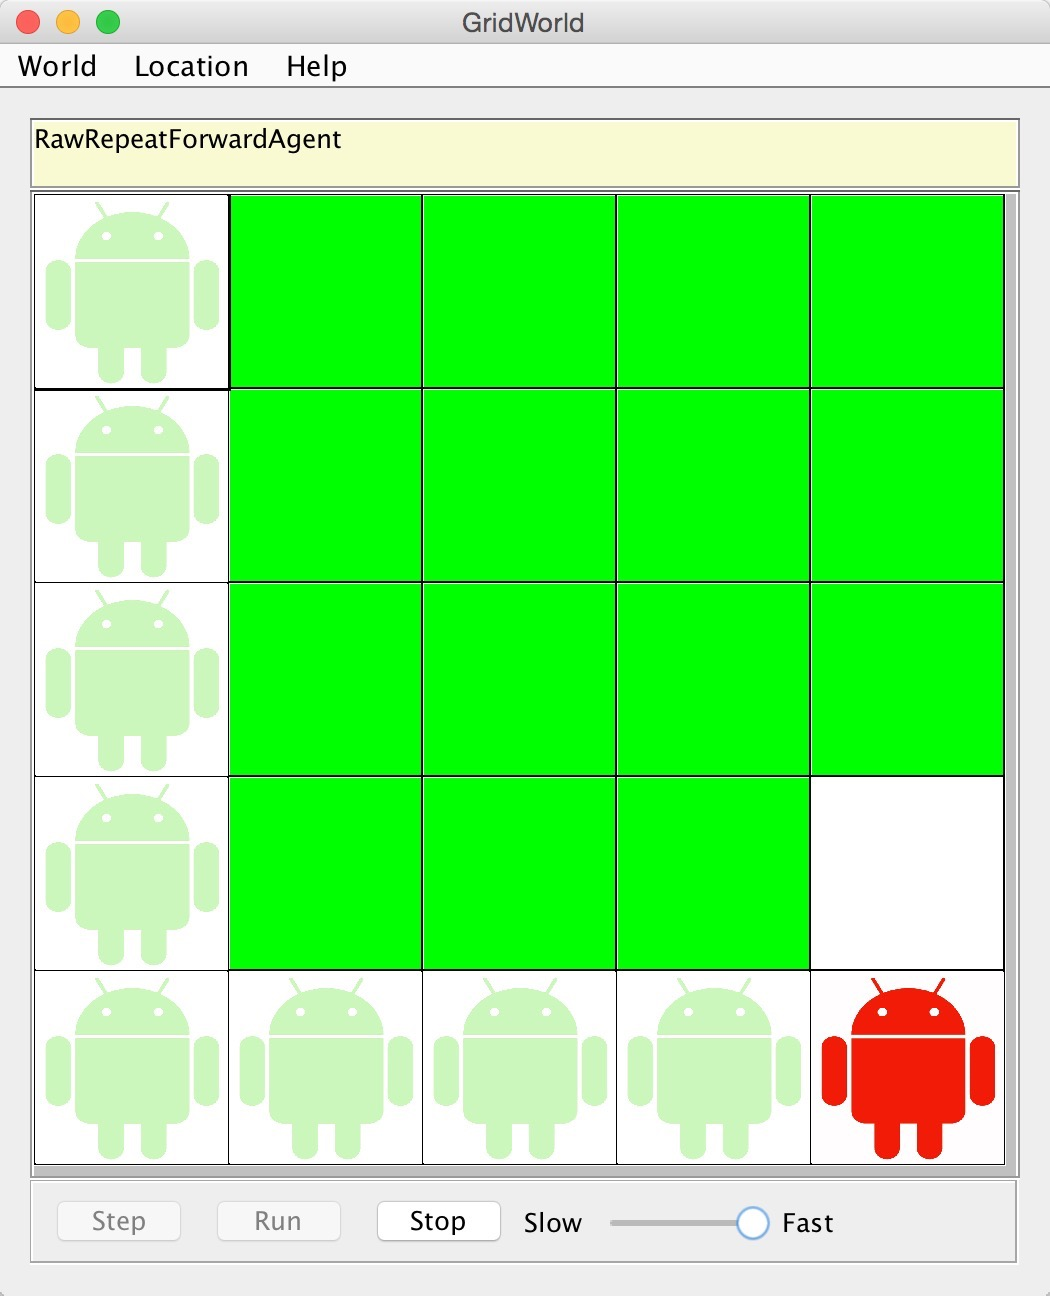
\includegraphics[width=\textwidth]{p2-rawforward}
    \caption{Raw RFA* breaking ties by $f$}
    \label{fig:rawforward}
  \end{subfigure}
  ~
  \begin{subfigure}[b]{0.30\textwidth}
    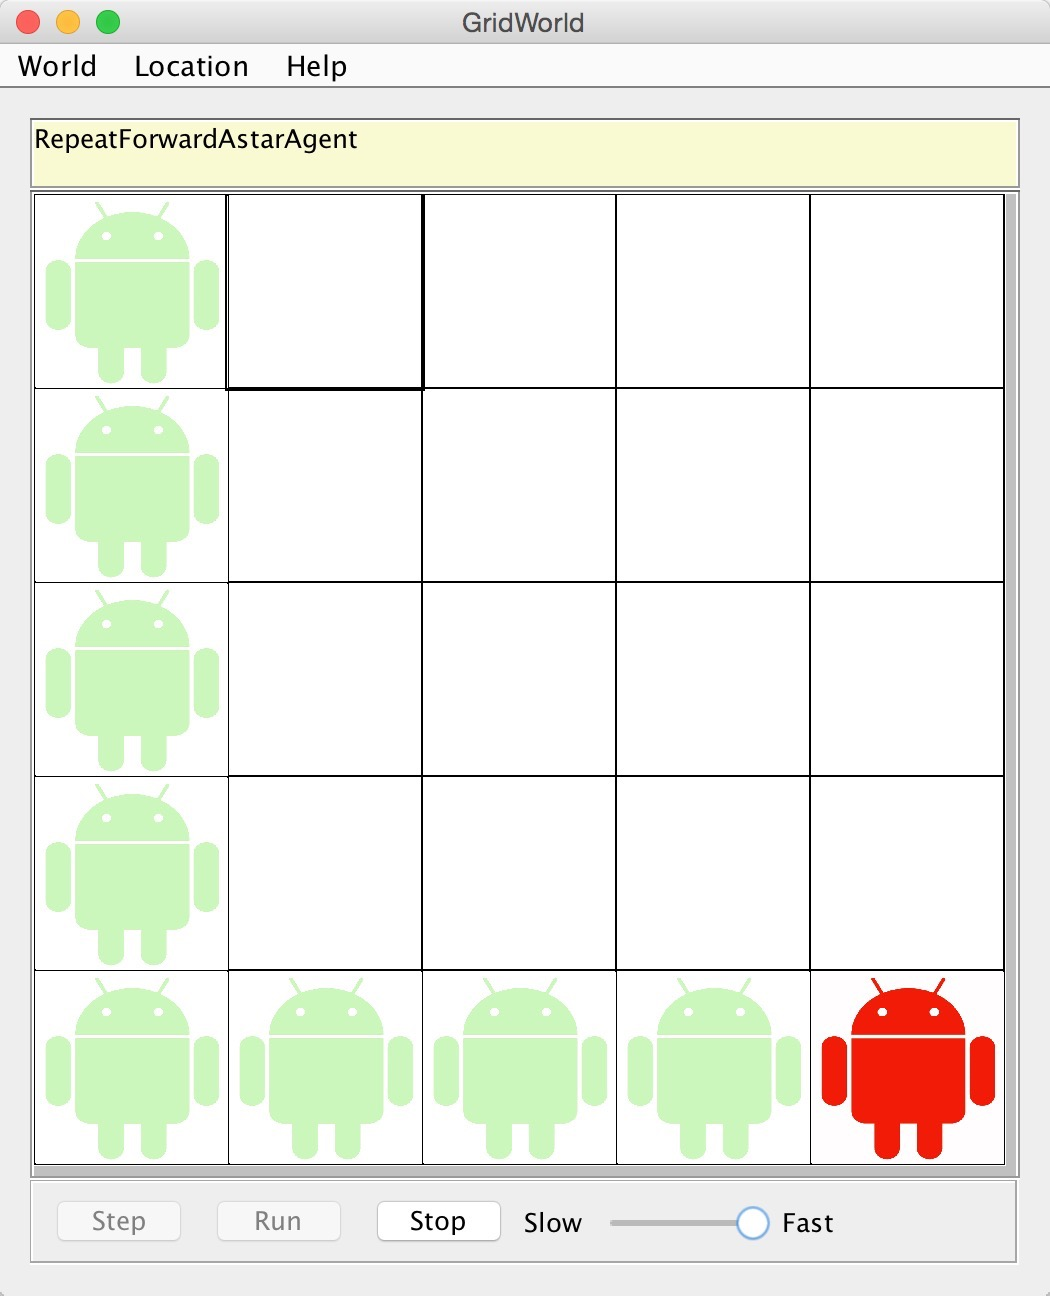
\includegraphics[width=\textwidth]{p2-newforward}
    \caption{Modified RFA* breaking ties by $(c\times f-g)$}
    \label{fig:newforward}
  \end{subfigure}
\caption{Results of two versions of Repeated Forward A*}
\end{figure}

